%\documentclass[12pt]{article}

\usepackage{epsfig,times,fullpage}

\documentclass[letterpaper,12pt]{article}

\usepackage{epsfig,times}





% typeblock size of 6.5 by 4 inches
\setlength{\textheight}{6.5in} \setlength{\textwidth}{4.5in}
\setlength{\oddsidemargin}{1in} \setlength{\evensidemargin}{1in} 
\setlength{\topmargin}{55.9pt} \setlength{\footskip}{27.5pt} 
\setlength{\headheight}{14.6pt} \setlength{\headsep}{19.9pt} 

% use this line for pre-runs of latex to generate correct TOCs and references
%\usepackage[noprint]{booklet}

% use this line for the final run to do the layout
\usepackage[print,1to1]{booklet} \nofiles 

%\pagespersignature{4}


\usepackage{ifpdf}
\ifpdf
  \setpdftargetpages
\else
  \setdvipstargetpages
\fi
\ifprintoption  % tweak dvi output only for final printing
  \special{!TeXDict begin /landplus90{true}store end}
  \special{!TeXDict begin <</Tumble true>> setpagedevice end}
\fi



% for dvips
%\special{landscape}



\newcommand{\gameName}{Nova Zembla}

\begin{document}

\thispagestyle{empty}
\begin{center}

~\vfill

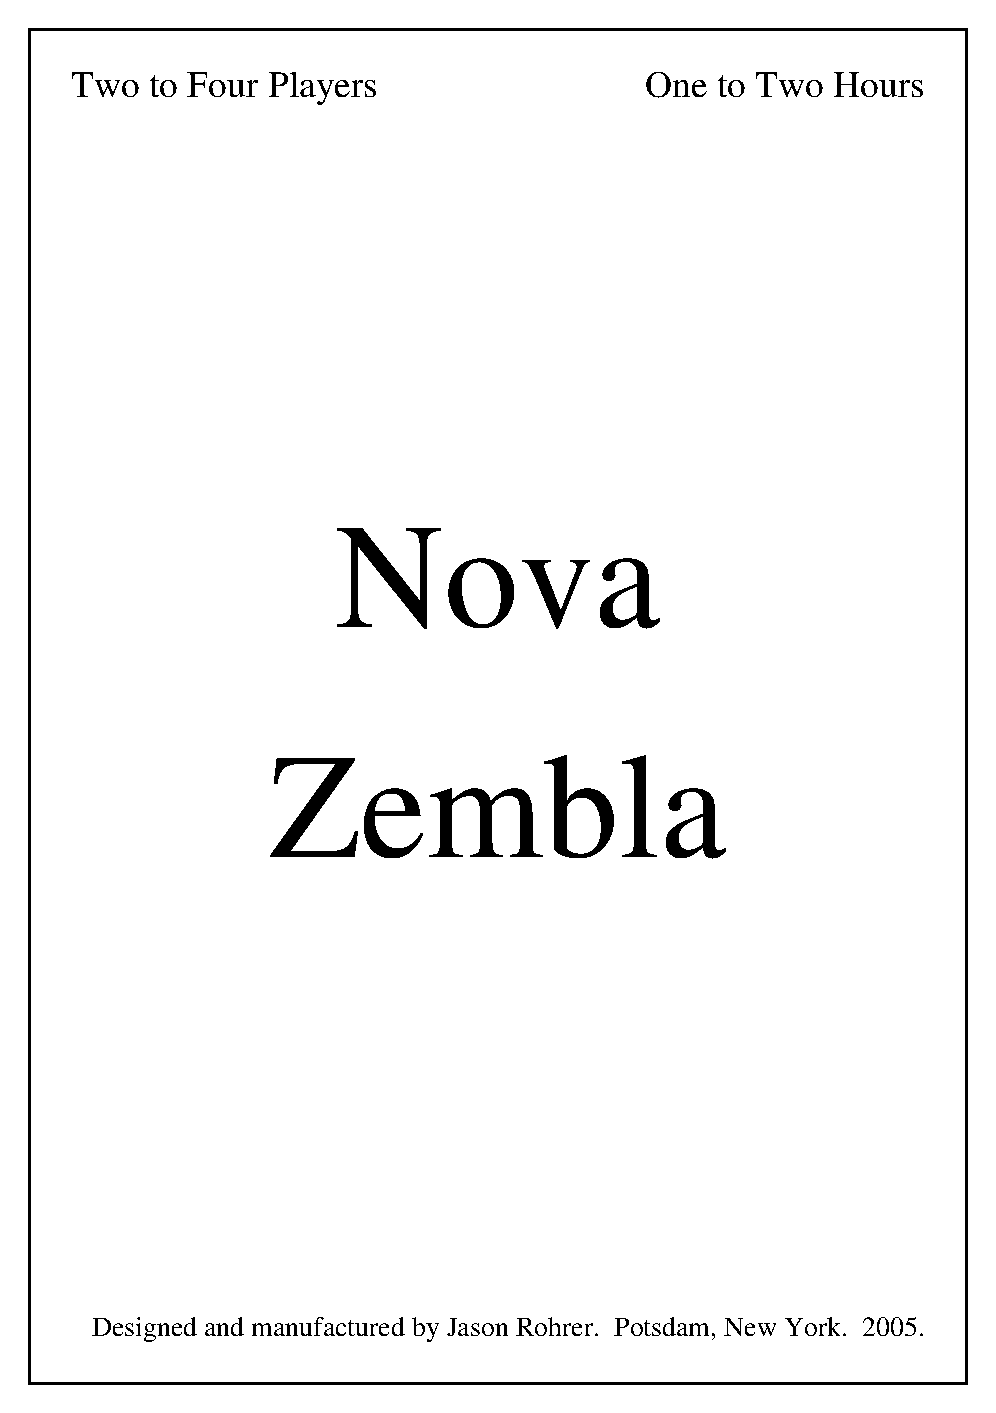
\includegraphics[width=0.98\textwidth]{rule_cover.eps}

\vfill

\end{center}



You and your opponents first work together to create a new world, a {\it nova zembla}.

You then each place a single believer in the world.
From that lone seed of belief, you try to grow your pool of believers to dominate the various regions of \gameName. 

However, the world you have created is fleeting.
After each turn, one small piece of the world is destroyed and scored, and you gain points if your believers hold the majority on that piece.
Thus, \gameName\ is constantly shrinking, and you must balance your need to establish believer-majority with the fact your believers on a given piece of the world will be destroyed when that piece is scored.

The game ends when the entire world has been destroyed.
If you have more points than your opponents, you win.


\section{Equipment}

\gameName\ includes the following components: 
\begin{itemize}
  \item one point track;
  \item 30 map tiles, including 8 cities and 22 countrysides;
  \item 200 pieces of kernel currency;
  \item 50 believer markers (beans) for each player; 
  \item one temple marker for each player;  and
\end{itemize}
Each map tile is marked on its corners with a point value.
When the tile is removed from the world, these points go to whichever player has the majority on the tile.

Cities have an additional population number (inside a black diamond).
If you hold the majority in a city, you get to add that many new believers to the city during your turn.

Countrysides have an additional kernel number (inside a circle).
If you hold the majority in a countryside, you get to collect that many kernels during your turn.



\section{Setup}


Each player starts the game without any kernels.  

The map tiles are spread out, face down, and shuffled.
The tiles are then collected, still face down, to form a random-ordered stack.
The stack is placed to one side of an empty playing surface.

Each player puts one believer marker on the point track's zero point.

Players draw straws to see who goes first.  Play continues clockwise. 



\section{World Creation}

\subsection{Map}
The first player picks a tile from the top of the face-down stack and places it, face up, in the center of the playing surface.  The next player then picks a tile and places it adjacent to the first tile.  Players continue taking turns, picking a tile and adding it adjacent to one of the tiles that is already part of the map.
The map can grow in any direction---the resulting map may have ``peninsulas'' and other irregular feature.

% FIXME: show image of possible map layout here

This process ends when all the tiles have been placed.

{\bf Note:}  a shorter game can be played by agreeing to stop after laying fewer than 30 tiles.
For example a 15-tile game would last approximately 30-60 minutes.

\subsection{Believers}
Starting again with the first player, players take turns placing their first believers on empty city tiles.
Each player must pick a different city, and first believers {\em cannot} be placed on countryside tiles.
After each placing a single believer, regular game rounds begin as described below.
Note that each player starts the game with a {\bf single believer} on the map.


\section{Game Rounds}

Nova Zembla play progresses through a series of rounds.
Each round is made up of an ordered sequence of seven steps.
Players take turns during each step before they move on to the next step.
Thus, the first player performs Step 1, followed by the second player, and so on.
Then the first player performs Step 2, followed by the second player, and so on.
After completing all seven steps together, players move on to the next round, starting again with Step 1.

The sequence of steps during each round can be summarized as follows:
\begin{center}
\begin{tabular}{|rrl|}
\hline
1.&{\bf Convert}& opponents' believers\\
\hline
2.&{\bf Attract}& believers to your temple\\
\hline
3.&{\bf Build}& your temple\\
\hline
4.&{\bf Collect}& 3 kernels, plus kernels from your countrysides\\
\hline
5.&{\bf Populate}& your cities with additional believers\\
\hline
6.&{\bf Move}& your believers\\
\hline
7.&{\bf Remove}& tiles from the map\\
\hline
\end{tabular}
\end{center}
For quick reference, these steps are listed on the the point track.
The details for each step are given below.
\begin{enumerate}

\item Players take turns {\bf converting} opponents' believers.
If you have a single believer on a tile containing one or more of your opponents' believers, you can pay five kernels to convert them.
The number you can convert is limited by the point value of the tile.
Thus, on a six-point tile, you can pay five kernels to convert up to six believers to your side (you pay a total of five kernels for the conversion, not five kernels per believer).
On a one-point tile, the same five kernels would allow you to convert only one believer.
The believers you convert can belong to more than one of your opponents.  
When you convert believers, you remove your opponents' believers and replace them with your own.
Removed believers are returned to your opponents' pools of believers.
You can pay to convert believers as many times as you want on a given turn in Step 1, but only on tiles where you still have only a single believer.
Your temple keeper can also perform conversions if it is your only believer on the tile.
You cannot convert any opponent's last believer.

\item Players take turns {\bf attracting} believers to their temples.
If you have a temple on the map, you {\em must} attract believers to it.
The number you attract depends on the point value of the tile where your temple is located and how many believers are already around your temple.
For example, on a six-point tile, you must attract believers on your turn until there are six around your temple.
If there are already six or more believers around your temple, you cannot attract more.
On a nine-point tile, you must attract believers each turn to maintain at least nine around your temple.
You can attract any mix of believers from other tiles, including your own believers.

\item Players take turns {\bf building} temples.
You can build your temple on any tile where you hold the majority and have enough believers for the required sacrifice.
The cost of the temple in kernels and believers equals the point value of the tile.
For example, to build on a six-point tile, you must pay six kernels and remove six of your believers from the tile.
One of the sacrificed believers must be placed in the temple as the temple keeper.
This temple keeper cannot be converted by your opponents or moved to another tile.
Your temple keeper does count toward your majority on the tile (thus, you always have at least one believer on the tile).
Also, the temple keeper can be used in Step 2 to convert opponents' believers. 
Only one temple can occupy each tile.

\item Players take turns {\bf collecting} kernels.
You {\em must} collect three kernels, plus extra kernels for each countryside tile where you hold the majority (collect the number of kernels listed in the circle on the tile).

\item Players take turns {\bf populating} their cities.
You {\em must} add believers to each city tile where you hold the majority (add the number of believers listed in the diamond on the tile).
There is no limit to how crowded a city can become as you continue adding believers during Step 5 in each round.

\item Players take turns {\bf moving} their believers.
During your turn, you can take either of the following movement actions any number of times and in any order:
\begin{itemize}
\item Pay one kernel to move one of your believers to an adjacent tile (no diagonal moves).
\item Pay four kernels to jump one of your believers across the map to any tile.
\end{itemize}
There is no limit to how many times you can move your believers during your turn.

\item Players take turns {\bf removing} tiles.
You {\em must} pick one tile from the map to remove and score.
There are two factors limiting the choice of a tile to remove:
\begin{itemize}
\item You cannot remove a tile that is completely fenced-in by other tiles (you must be able to slide the tile out of the map without lifting it over other tiles).
\item You cannot remove a tile containing a player's last believer, unless there is no other choice.
\end{itemize}
The player who holds the majority on the tile gains points when that tile is removed, as described below in Section \ref{sec:scoring}.
Believers and temples on the tile are returned to their respective owners.
A player's temple, once removed, can be rebuilt on another tile during Step 3 in a future round.
\end{enumerate}




\subsection{Scoring a tile}
\label{sec:scoring}
When a tile is removed, the player that has the majority of believers on the tile gains the number of points listed on the corners of the tile.
If no player has the majority, including the case of a tie, no player gets points when the tile is scored.

If a temple is present on the tile, the tile is worth twice as many points for whoever has the majority, even if the majority is held by a player that does not own the temple.

\subsection{Game end}

When the last tile has been removed, the game is over.
The player with the highest score on the point track is the winner.
Ties are possible.


\section{What if...?}

\paragraph{Running out of believers} If you have all of your 50 believer markers on the map, you cannot add any more until some are removed from the map.
Thus, you must skip the {\bf Convert} and {\bf Populate} steps.

\paragraph{Removing a players' last believer} According to the rules above, you can only remove a tile containing a player's last believer if you have no other choice.
In fact, this can only happen near the end of the game (where each remaining tile contains some player's last believer).
Thus, it is possible for players to get knocked out of the game at the end.
Players that have no believers left on the map must skip their turn, though they can still bid to remove tiles from the map during the auctions at the end of the remaining players' turns.
 
\end{document}